\section{Modeling a truncated prediction}
\label{sec:trunc_modelling}

Both the usual truncation schemes, linear and quadratic, are covered by the tools discussed so far ($A$-coefficients/ELR and MM). The former keeps only the SM interference with dimension-six operators at the cross section level, therefore neglecting all terms of order $1/\Lambda^4$. The later defines the expansion at the amplitude level, $\mathcal{M}=\mathcal{M}_{\text{SM}}+\mathcal{M}_{\text{dim6}}$, therefore carrying terms of order $|\mathcal{M}_{\text{dim6}}|^2\sim1/\Lambda^4$ at the cross section level---but missing terms originating from SM times double dimension-6 insertions, $\sigma_{\text{SM}\times\text{dim6}^2}\sim\mathcal{O}(1/\Lambda^4)$, an additional interference that would require contributions from dimension-8 operators. The caveat of adding subleading operators is that those have an extra loop suppression and therefore contribute only linearly in the cross section. In this regard power counting-wise, the quadratic components of the subleading operators are closer to the contributions coming from the first dimension-8 contributions, similarly to the double insertion of leading operators. 

As reference, we generate some of the benchmarks discussed in Ref.~\cite{Bär:2965348} with the PDF set \texttt{PDF4LHC\_21} in both truncations, and compare the results obtained from the $A$-coefficients and by the MM approach. The resulting distributions are shown in Figure \ref{fig:linearquad}. The linear truncation is achieved by switching off the $A$-coefficients related to the quadratic components shown in Table \ref{fig:linearquad}. For the MM, the basis samples were generated with the linear truncation and solved the coefficients bin by bin, restricting the sum to the ten linear monomials at evaluation. The total
cross sections agree with the simulation to $1.3$--$2.2\%$ at BM1 and BM2 and to $3.5\%$
at BM5, in the quadratic and in the linear truncation. At BM4 the linearly truncated
prediction is negative, $-0.045$~pb against $-0.041$~pb in the generated sample, whose
event weights are negative in $98\%$ of events, so the method follows the truncation into
that region as well. 


%Sec.~\ref{sec:truncation} states over what range of the Wilson coefficients a chosen
%dimension-6 truncation is one an analysis would want. This section asks the separate
%question of whether the tools of this report reproduce that truncation once it is chosen:
%whether a prediction truncated at the interference term, or at the leading quadratic
%terms, is described as well as the complete one, by the reweighting evaluated directly and
%by the matrix method on the optimized basis alike. Both are needed, because an analysis
%quoting a linear result has to produce it with the same machinery it uses for everything
%else.

%The truncation is the choice of which powers of $1/\Lambda^2$ are kept in the polynomial.
%The results of this report use the quadratic truncation for the leading operators and the
%linear one for the subleading operators, the option \texttt{b} of \texttt{POWHEG-BOX-V2}
%combined with $\textsc{includesubleading}==1$ of Sec.~\ref{sec:parameterization}. That
%choice fixes both the normalization and the \mHH and \pt shapes away from the SM point,
%by an amount that grows with the Wilson coefficients and, for the operators that generate
%energy-growing amplitudes, with the momentum transfer.

%The study needs no additional coefficient fit. Eq.~\eqref{eq:smeftpara_reorg} \emph{is} the
%truncated cross section, organized bracket by bracket in
%Table~\ref{tab:smeft_matrix_blocks}, so a change of truncation amounts to including or
%dropping one group of $A$-coefficients. All 40 coefficients have already been extracted,
%per bin and at each energy (Sec.~\ref{sec:extraction}), and every truncation is a different
%subset of the same 40 numbers. The only simulated input entering this section is the set of
%benchmark samples described below.

%\textcolor{red}{DEFERRED to Sec.~\ref{sec:energy_beyond}: the inclusive ratio
%$\sigma_{\text{trunc}}/\sigma_{\text{nom}}$ along one-dimensional rays, and the same
%ratio differentially, are better shown at the two energies together than at $13.6$~TeV
%alone. The $13.6$~TeV halves can be produced today from the $A$-coefficients fitted to
%the generated samples; the $100$~TeV halves wait on that extraction.}

%Three predictions are compared, all read off the same coefficient set. The \emph{linear}
%one keeps the SM term $A^j_0$ with the linear brackets only, the leading terms
%$A^j_1$--$A^j_4$ and the subleading terms $A^j_{15}$--$A^j_{19}$; it is the strictly
%dimension-6 interference prediction. The \emph{leading-quadratic} one adds the leading-only
%quadratic block $A^j_5$--$A^j_{14}$. The \emph{nominal} one adds the
%leading$\,\times\,$subleading block $A^j_{20}$--$A^j_{39}$ and is the truncation used
%throughout this report. The only dimension-6 squared terms absent from all three are the
%purely subleading squares, dropped in the generation (Sec.~\ref{sec:parameterization});
%they are not accessible from these coefficients.

%Ref.~\cite{Bär:2965348} defines a set of \HH benchmark points in the same operator space
%and provides, for each, a prediction generated separately in the linear and in the
%quadratic truncation. They are an external test rather than two evaluations of one fit: each truncated
%prediction is compared with the simulation produced with that truncation, so an error in
%the bracket bookkeeping would appear in one truncation while the other still closed. Four of them are used here, defined
%y $c_\PH=3$; $c_\PH=-2$, $c_{\PH\mathrm{kin}}=-2$, $c_{\PQt\PH}=4$; $c_\PH=-6$; and
%$c_\PH=-3$, $c_{\PH\mathrm{kin}}=-2$, $c_{\PQt\PH}=0.5$, all other coefficients at zero.

%The comparison is shown in Fig.~\ref{fig:linearquad}. In each panel the polynomial
%reproduces the generated spectrum in the linear and in the quadratic truncation alike, so
%the $A$-coefficients describe not only the nominal prediction but each of its truncations
%separately. The same holds for the other route. Taking the forty-point basis with its templates from
%the generated samples, solving for the coefficients bin by bin and restricting the sum to
%the ten linear monomials at evaluation reproduces the same generated spectra: the total
%cross sections agree with the simulation to $1.3$--$2.2\%$ at BM1 and BM2 and to $3.5\%$
%at BM5, in the nominal and in the linear truncation alike. At BM4 the linearly truncated
%prediction is negative, $-0.045$~pb against $-0.041$~pb in the generated sample, whose
%event weights are negative in $98\%$ of events, so the method follows the truncation into
%that region as well. Both tools therefore model each truncation, and both close against
%simulation when truncated as they do when complete.

%These benchmark samples were generated with \texttt{PDF4LHC21\_40}, a newer set
%than the \texttt{PDF4LHC15\_nlo\_30\_pdfas} used for the samples the coefficients were
%fitted from (Sec.~\ref{sec:eventsimulation}), and the panels close over the whole \mHH
%range notwithstanding. The reweighting is a ratio of cross sections evaluated at
%the same kinematics, so a change of parton densities largely cancels in it, and the
%closure across two different sets measures what does not cancel. The separation between the two sets of
%curves within a panel is the truncation effect itself, at coupling values of order a few.
%The benchmark at $c_\PH=-6$ shows the other practical consequence of truncating at the
%interference term: a strictly linear cross section is of first degree in the Wilson
%coefficients and carries no positivity guarantee once the interference overwhelms the
%SM term, and the vertical scale of that panel accordingly reaches negative
%values.

\begin{figure}[t]
  \centering
  \begin{minipage}[b]{0.495\linewidth}
    \centering
    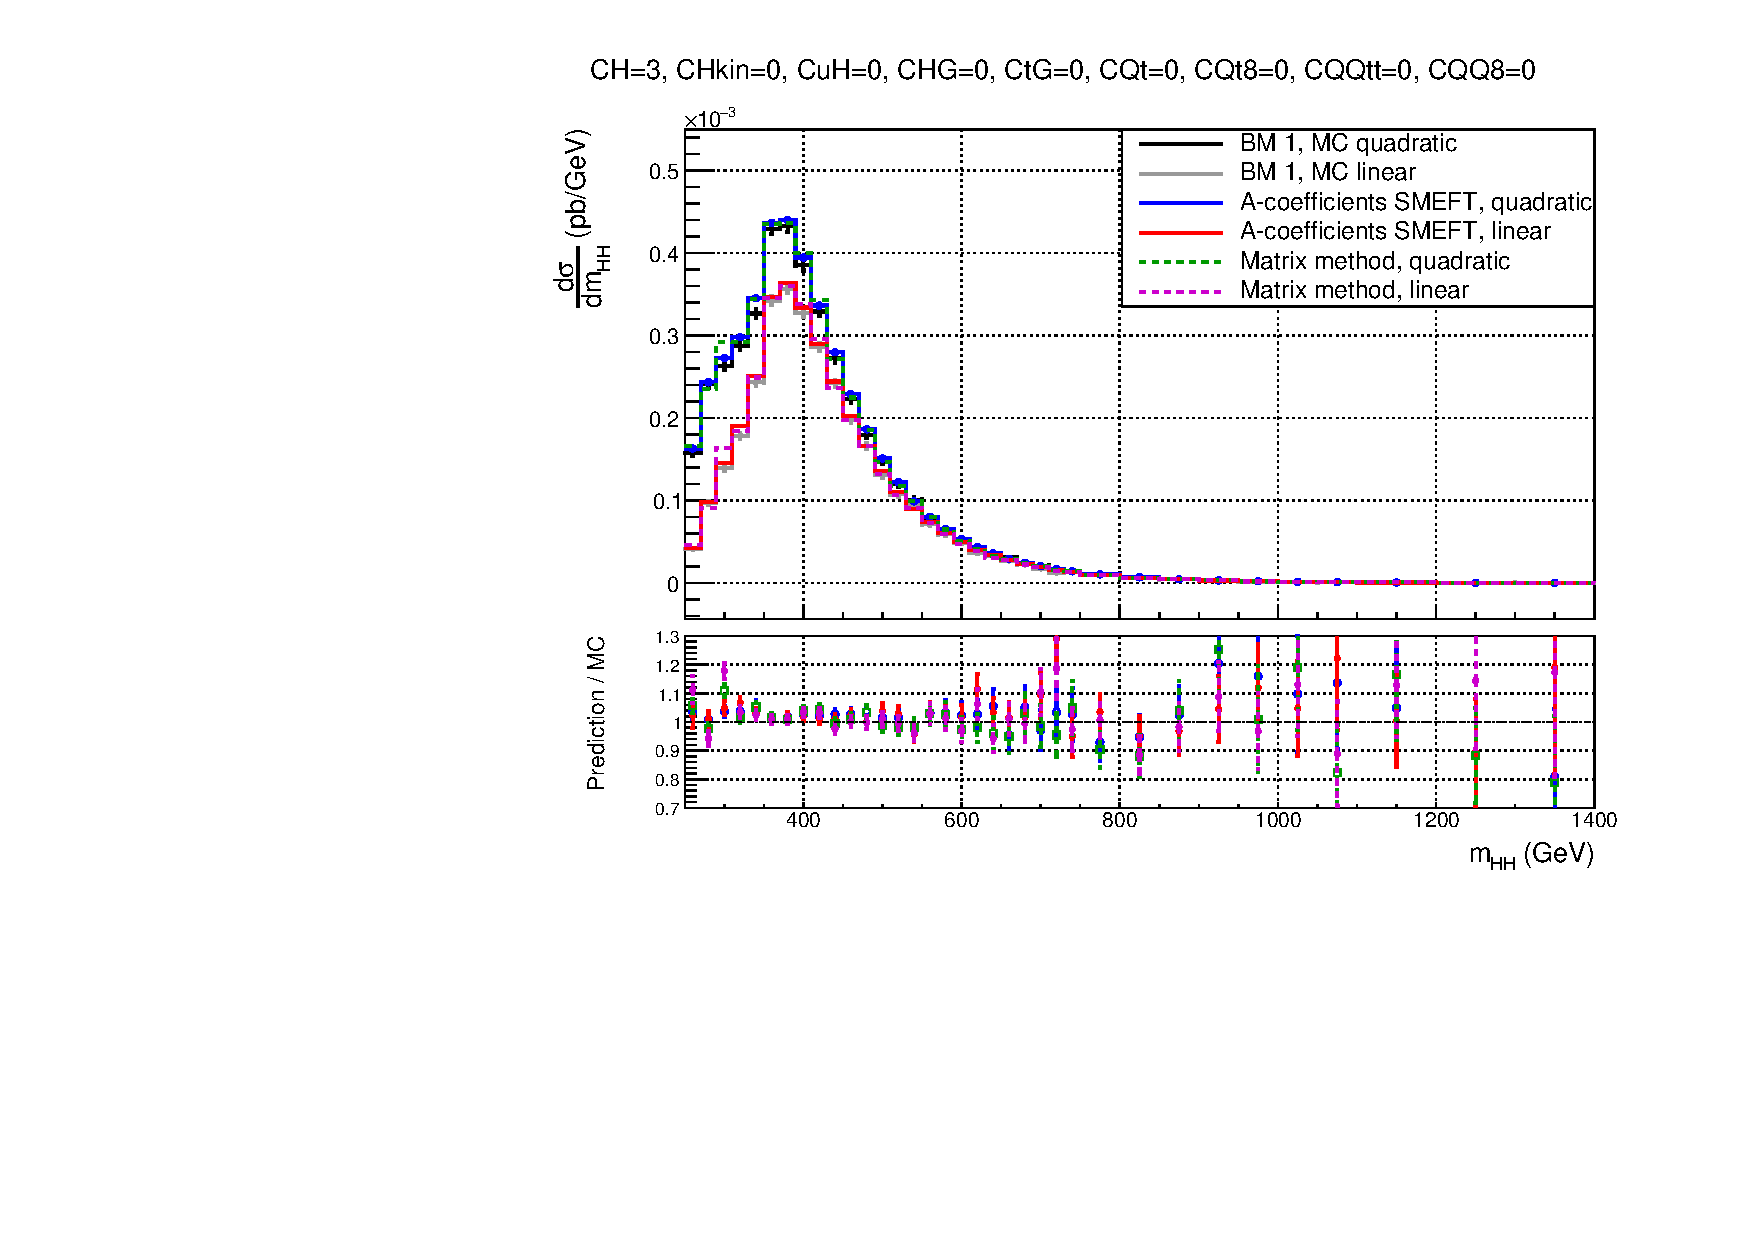
\includegraphics[width=\linewidth]{plots/poly_3d_9D_trunc_linvsquad_MM_(5)_CH_3.0_CHbox_0.0_CuH_0.0_CHG_0.0_CtG_0.0_CQt_0.0_CQt8_0.0_CQQtt_0.0_CQQ8_0.0.pdf}
  \end{minipage}
  \hfill
  \begin{minipage}[b]{0.495\linewidth}
    \centering
    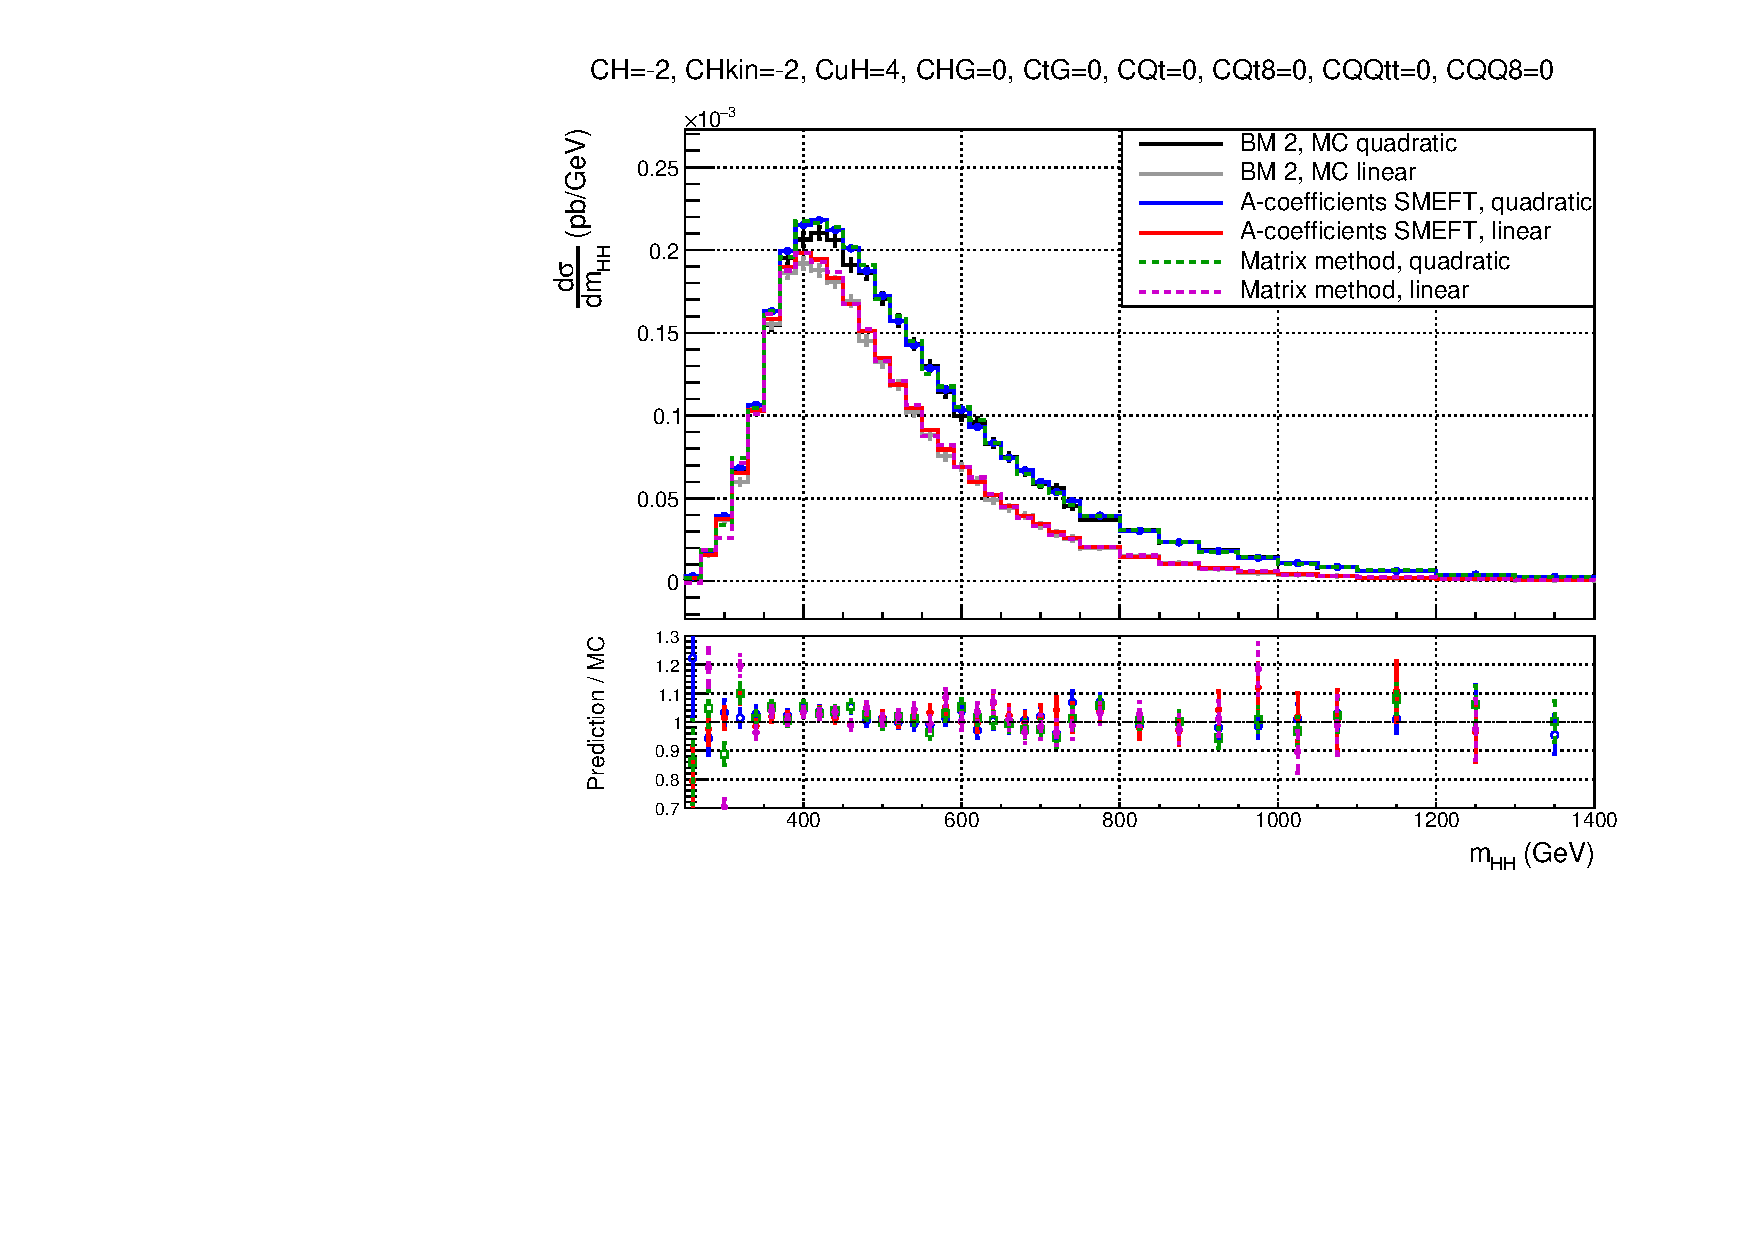
\includegraphics[width=\linewidth]{plots/poly_3d_9D_trunc_linvsquad_MM_(4)_CH_-2.0_CHbox_-2.0_CuH_4.0_CHG_0.0_CtG_0.0_CQt_0.0_CQt8_0.0_CQQtt_0.0_CQQ8_0.0.pdf}
  \end{minipage}
  \vspace{0.5em}
  \begin{minipage}[b]{0.495\linewidth}
    \centering
    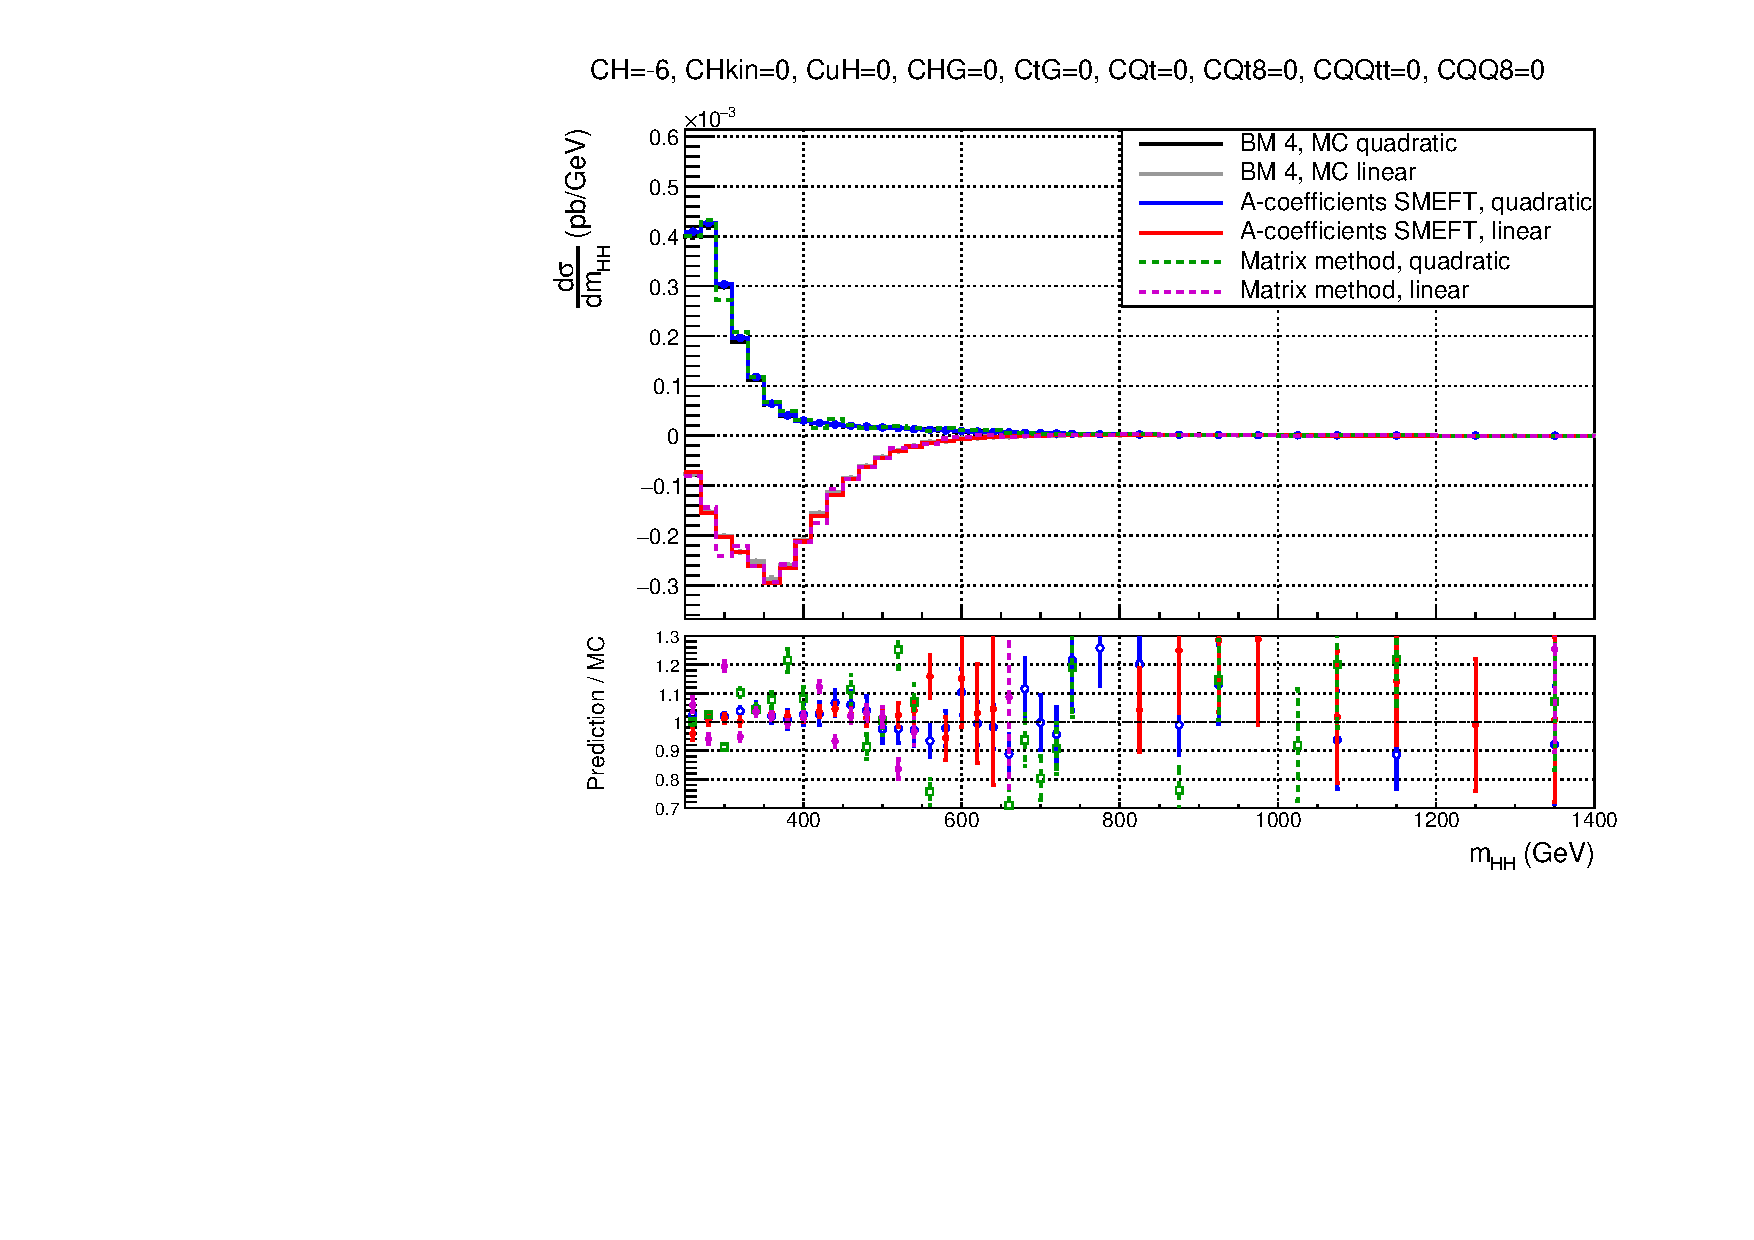
\includegraphics[width=\linewidth]{plots/poly_3d_9D_trunc_linvsquad_MM_(1)_CH_-6.0_CHbox_0.0_CuH_0.0_CHG_0.0_CtG_0.0_CQt_0.0_CQt8_0.0_CQQtt_0.0_CQQ8_0.0.pdf}
  \end{minipage}
  \hfill
  \begin{minipage}[b]{0.495\linewidth}
    \centering
    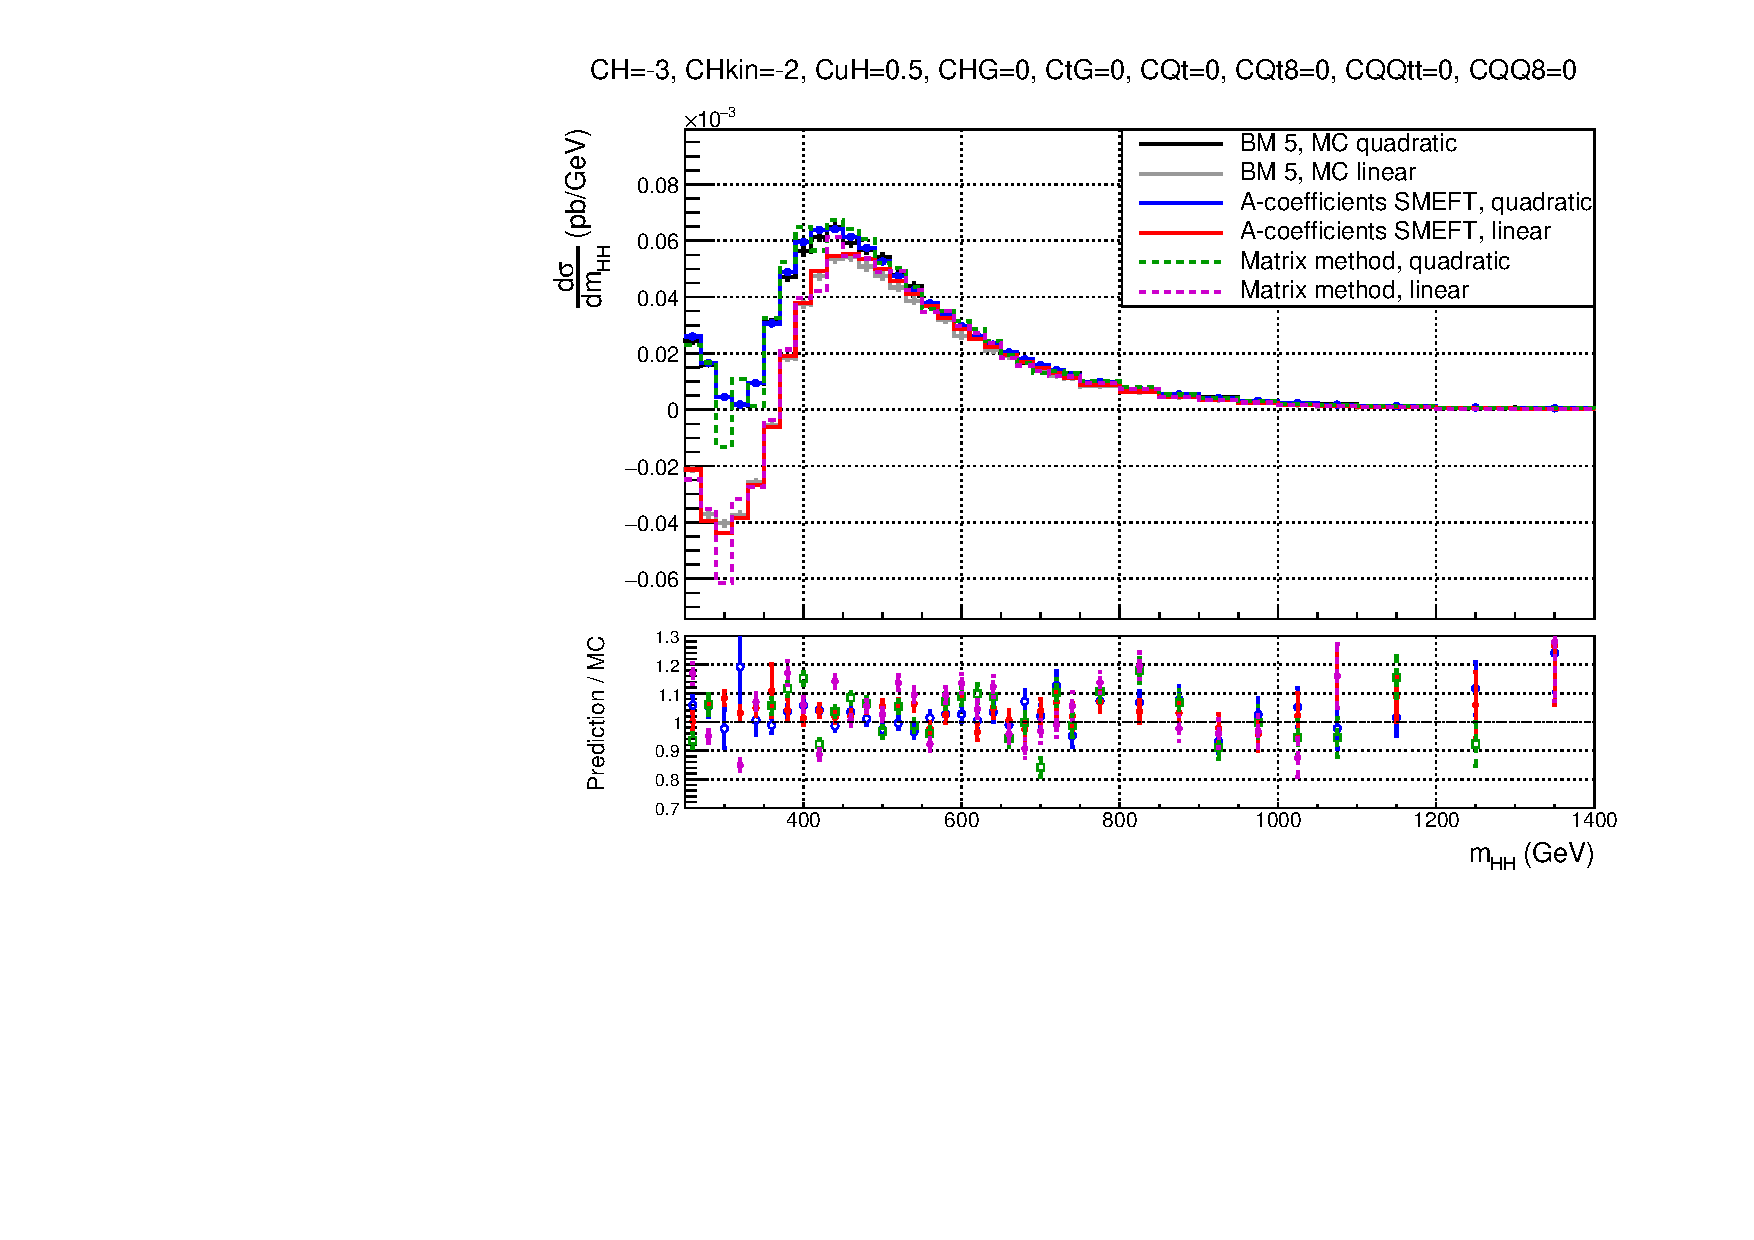
\includegraphics[width=\linewidth]{plots/poly_3d_9D_trunc_linvsquad_MM_(2)_CH_-3.0_CHbox_-2.0_CuH_0.5_CHG_0.0_CtG_0.0_CQt_0.0_CQt8_0.0_CQQtt_0.0_CQQ8_0.0.pdf}
  \end{minipage}
  \caption{Differential cross section in \mHH for four of the benchmark points defined in Ref.~\cite{Bär:2965348}: BM~1, $c_\PH=3$ (top left); BM~2, $c_\PH=-2$, $c_{\PH\mathrm{kin}}=-2$, $c_{\PQt\PH}=4$ (top right); BM~4, $c_\PH=-6$ (bottom left); and BM~5, $c_\PH=-3$, $c_{\PH\mathrm{kin}}=-2$, $c_{\PQt\PH}=0.5$ (bottom right). All other Wilson coefficients are zero. Each panel shows the samples generated at that point in the linear and in the quadratic truncation, together with the corresponding predictions of the 3D $A$-coefficient parameterization projected onto \mHH and the results obtained from MM. The lower pad gives the ratio of the parameterization to the simulation.}
%\textcolor{red}{The matrix-method curves, nominal and linearly truncated, are still to
%be overlaid on these panels; the request and the location of the histograms are in the
%text below. This sentence comes out once the curves are in.}}
  \label{fig:linearquad}
\end{figure}

% --- three figures still to be produced; the request is in the text above ---
% \newcommand{\truncplaceholder}[1]{%
%   \fbox{\begin{minipage}[c][0.26\textheight][c]{0.86\textwidth}\centering
%   \textcolor{red}{\textbf{[FIGURE PLACEHOLDER]}\\[4pt] #1}\end{minipage}}}
%
% \begin{figure}[ht]
% \centering
% \truncplaceholder{Inclusive cross-section ratio $\sigma_{\text{trunc}}/\sigma_{\text{nom}}$, for the linear and the leading-quadratic truncation over the nominal one, as a function of each Wilson coefficient along one-dimensional rays, at $13.6$~TeV.}
% \caption{\textcolor{red}{PLACEHOLDER. Inclusive truncation ratio as a function of each Wilson coefficient, built from the extracted $A$-coefficients.}}
% \label{fig:trunc_inclusive}
% \end{figure}
%
% \begin{figure}[ht]
% \centering
% \truncplaceholder{Differential truncation ratio in \mHH (left) and \pt (right), for a few representative points along the rays of Fig.~\ref{fig:trunc_inclusive}.}
% \caption{\textcolor{red}{PLACEHOLDER. Differential truncation ratio in \mHH and \pt, from the per-bin $A$-coefficients.}}
% \label{fig:trunc_diff}
% \end{figure}
%
% \begin{figure}[ht]
% \centering
% \truncplaceholder{Coupling range over which the linear and the nominal predictions agree to within a chosen tolerance, shown for each Wilson coefficient at $13.6$ and at $100$~TeV.}
% \caption{\textcolor{red}{PLACEHOLDER. Comparison of the truncation validity range at the two energies.}}
% \label{fig:trunc_energy}
% \end{figure}

%An analysis that wants the interference-only prediction therefore needs no separate set of
%samples: the forty templates are untruncated distributions and the truncation is applied
%when the formula is evaluated. Fitting the ten-term system directly instead does not
%reproduce samples generated with that truncation, and a dedicated ten-point basis was
%built and is not recommended, for reasons given in Sec.~\ref{sec:validation_realistic}.

%\textcolor{red}{\textbf{MATHEUS:} we are condensing the truncation material into this
%one comparison, so that a single figure shows that every truncation of the
%parameterization can be modelled --- the reweighting evaluated directly, and the
%matrix-method basis with the formula truncated at evaluation --- rather than one figure
%per route. Could the matrix-method curve be added to the four panels of
%Fig.~\ref{fig:linearquad}? \textbf{The histograms are ready} at
%\texttt{/eos/user/a/acarvalh/to\_Matheus/mm\_truncation\_benchmarks\_13p6TeV.csv}, with a
%README and the handover note beside it, in the binning of Table~\ref{tab:binedge} so the
%edges match your axes. They are the matrix method on the generated basis, nominal and
%linearly truncated, against the generated benchmark samples, with the closure quoted
%above. Please keep the BM4 panel as it comes out, negative axis included: it is where the
%linear truncation has left its validity range and the method still follows it.}
